\documentclass{article}
\usepackage{tikzpeople}
\usepackage{tikz}
\usetikzlibrary{shapes, shapes.misc}
\usetikzlibrary{arrows, arrows.meta, decorations.markings}
\usetikzlibrary{patterns}

\begin{document}
\begin{center}
\resizebox{\columnwidth}{!}{%
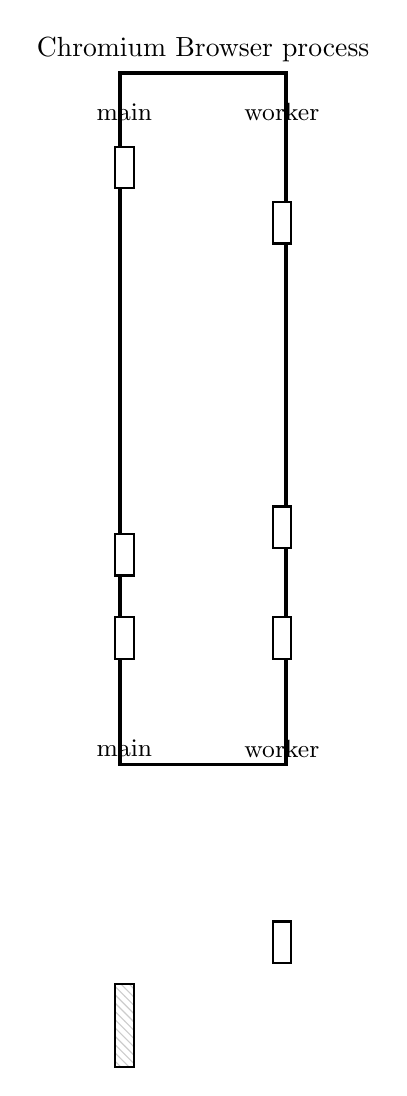
\begin{tikzpicture}[>=latex]
%\tikzstyle{every node}=[font=\Large]
\tikzstyle{app} = [draw, very thick, minimum height=250pt, minimum width=60pt, fill=white, rectangle, font={\sffamily\bfseries}]
\tikzstyle{appbegin} = [minimum width = 10pt, below = -240pt of #1]
\tikzstyle{append} =[minimum width = 10pt, below = -10pt of #1]
\tikzstyle{thread} = [minimum width = 4pt, font=\small]

\tikzstyle{actionpoint} = [draw, thick, minimum width = 5pt, minimum height = 15pt, fill = white]
\tikzstyle{blocked} = [minimum height = 15pt, pattern=north west lines, pattern color = black!40!, font=\scriptsize, rotate=270] 
\tikzstyle{blockedactionpoint} = [draw, thick, minimum width = 5pt, minimum height = 30pt, pattern=north west lines, pattern color = black!20!] 

\tikzstyle{point} = [thick, draw=red, cross out, inner sep = 0pt, minimum width = 3pt, minimum height =3pt]
%\tikzset{
%%ext/.pic={
%%\path [fill=white] (-0.2,0)to[bend left](0,0.1)to[bend right](0.2,0.2)to(0.2,0)to[bend left](0,-0.1)to[bend right](-0.2,-0.2)--cycle;
%%\draw (-0.2,0)to[bend left](0,0.1)to[bend right](0.2,0.2) (0.2,0)to[bend left](0,-0.1)to[bend right](-0.2,-0.2);
%%},
%point/.style={
%    thick,
%    draw=red,
%    cross out,
%    inner sep=0pt,
%    minimum width=4pt,
%    minimum height=4pt,
%}}

%draw applications
%%browser
\node [app, name = browser, label=above:Chromium Browser process]{};
\node(browserbegin) [appbegin=browser]{};
\node(browserend) [append=browser]{};
\node (bt1begin)[thread, left of = browserbegin]{main};
\node (bt1end)[thread, left of = browserend]{main}; 
\node (bt2begin)[thread, right of = browserbegin]{worker};
\node (bt2end)[thread,  right of = browserend]{worker};

\node (1)[actionpoint, below of = bt1begin, node distance = 20pt]{};
\node (10)[actionpoint, below of = 1, node distance = 140pt]{};
\node (11)[actionpoint, below of = 10, node distance = 30pt]{};
\node (20)[blockedactionpoint, below of = 11, node distance = 140pt]{};

\node (2)[actionpoint, below of = bt2begin, node distance = 40pt]{};
\node (9)[actionpoint, below of = 2, node distance = 110pt] {};
\node (12)[actionpoint, below of = 9, node distance = 40pt]{};
\node (19)[actionpoint, below of = 12, node distance = 110pt] {};


%\draw [solid] (bt1begin) -- (1.north);
%\draw [solid] (1.south) -- (10.north);
%\draw [dotted] (10.south) -- (bt1end);
%\draw [solid] (bt2begin) -- (2.north);
%\draw [solid] (2.south) -- (9.north);
%\draw [solid] (9.south) -- (bt2end);
%
%%%renderer
%\node [app, name = renderer, right of = browser, node distance = 150pt]{Chromium Renderer Process};
%
%\node (rderbegin)[appbegin = renderer]{};
%\node (rderend)[append = renderer]{};
%
%\node (rt3begin)[thread, left of = rderbegin]{worker};
%\node (rt3end)[thread, left of = rderend]{worker};
%\node (rt4begin)[thread, right of = rderbegin]{main};
%\node [draw, below right = 9pt and 0.5pt of rt4begin, font=\scriptsize, rotate=270] {EventQueue};
%\node (rt4end)[thread, right of = rderend]{main};
%%\draw [solid] (bt3begin) -- (bt3end);
%%\draw [solid] (bt4begin) -- (bt4end);
%\node (3)[actionpoint, below of = rt3begin, node distance = 60pt]{};
%\node (4)[actionpoint, below of = rt4begin, node distance = 80pt]{};
%\node (7)[blockedactionpoint, below of = 4, node distance = 50pt]{};
%\node (12)[blocked, below right = -2pt and 10pt of 7]{semaphore wait};
%\node (8)[actionpoint, below of = 3, node distance = 80pt]{};
%\draw[solid] (rt3begin) -- (3.north);
%\draw[solid] (3.south) -- (8.north);
%\draw[solid] (8.south) -- (rt3end);
%\draw[solid] (rt4begin) -- (4.north);
%\draw[solid] (4.south) -- (7.north);
%\draw[dotted] (7.south) -- (rt4end);
%%
%\node [app, name = fontd, minimum width=40pt, right of = renderer, node distance = 100pt, label=above:fontd]{};
%\node (fontdbegin)[appbegin =fontd] {};
%\node (fontdend)[append = fontd]{};
%\node (ft5begin)[thread, left = -10pt of fontdbegin]{};
%\node (ft5end)[thread, left = -10pt of fontdend]{};
%\node (5)[actionpoint, below of = ft5begin, node distance = 90pt] {};
%\node (6)[below of = 5, node distance = 3pt] {};
%%\draw [solid] (bt5begin) -- (bt5end);
%%
%\node[draw, dotted, above left = -120pt and -300pt of browser, pattern=dots, pattern color = black!20!, minimum width =300pt, minimum height=80pt, label=below:flow of TextInputClientMsg FirstRectForCharacterRange]{};
%\node[draw, dotted, above left = -40pt and -170pt of 9, pattern=dots, pattern color = black!20!, minimum width =180pt, minimum height=60pt, label=below:flow of Javascript running]{};
%
%\draw [->] (1) -- (2);
%\draw [->] (2) -- (3);
%\draw [->] (3) -- (4);
%\draw [->] (4) -- (5);
%\coordinate[name = notarrive7, point, below right = 10pt and 10pt of 7]{};
%\draw [->] (6.west) -- (notarrive7);
%\coordinate[name = before7, above of = 7, node distance = 10pt]{};
%\draw [->] (before7) -- (8);
%\draw [->] (8) -- (9);
%\coordinate[name = notarrive10, point, below right = 10pt and 10pt of 10]{};
%\draw [->] (9) -- (notarrive10);
%%
%%\node (findfirstrect)[minimum width = 40pt, minimum height = 40pt, right of = 2, node distance = 50pt, rotate= 343] {TextInputClientMsg FirstRectForCharacterRange};
%%\node (javascript)[minimum width = 20pt, minimum height = 20pt, below left = 0pt and 5pt of 7, rotate = 15] {Run\_Javascript};
%
%\node(legend)[above right = 40pt of fontdend]{};
%\node (l1)[below left = -20pt and -20pt of legend] {};
%\node (l2)[right=8pt of l1]{};
%\draw [-, solid] (l1.east) -- (l2);
%\node [right= 10pt of l1, font=\large]{thread\_running};
%
%\node (l3)[below left = -30pt and -20pt of legend] {};
%\node (l4)[right=8pt of l3]{};
%\draw [-, dotted] (l3.east) -- (l4);
%\node [right =10pt of l3, font=\large]{thread\_wait};
%
%\node (l5)[below left = -40pt and -20pt of legend] {};
%\node (l6)[right =8pt of l5]{};
%\draw [->] (l5.east) -- (l6);
%\node [right =10pt of l5, font=\large]{IPC (edge)};
%
%\node [draw, solid, minimum width = 10pt, minimum height = 3pt, below left = -50pt and -30pt of legend, label={[font=\large]right:execution segment in thread(vertex)}]{};

\end{tikzpicture}
}
\end{center}
\end{document}
